\fenicschapter{FErari: an optimizing compiler for variational forms}
              {FErari: an optimizing compiler for \\ variational forms}
              {FErari: an optimizing compiler for variational forms}
              {Robert C. Kirby and Anders Logg}
              {kirby-3}

In Chapter~\ref{chap:kirby-8}, we presented a framework for efficient
evaluation of multilinear forms based on expressing the multilinear
form as a special tensor contraction. This allows generation of
efficient low-level code for assembly of a range of multilinear
forms. Moreover, in Chapter~\ref{chap:kirby-4} it was shown that the
tensor contraction may sometimes possess a special structure that
allows the contraction to be performed in a reduced number of
arithmetic operations. This has led to the FErari project
\citep{KirbyKnepleyLoggEtAl2005,KirbyLoggScottEtAl2006,KirbyScott2007,KirbyLogg2008},
which provides an option within the form compiler FFC described
in Chapter~\ref{chap:logg-1} to apply graph-based optimizations at
compile-time. In this chapter, we describe the interface between FFC and
FErari and present empirical results indicating the practical effect of
the FErari optimizations on run-time evaluation of variational forms. In
particular, we study the effect of optimizations on the run-time cost
of forming the cell tensor~$A_T$ defined in Chapter~\ref{chap:kirby-5}.

Before proceeding, it is important to put these optimizations in the
proper context. While FErari does not reduce the overall order of
complexity of finite element calculations, it provides a practical
benefit of reducing run-time from a few percent to sometimes tens of
percent. Viewed as a domain-specific compiler optimization, this is
quite respectable.

%------------------------------------------------------------------------------
\section{Optimized form compilation}

FFC supports two different modes of code generation depending on how
the multilinear form is represented. A user may select the tensor
representation $A_T = A^0 : G_T$ discussed in
Chapter~\ref{chap:kirby-8} by supplying the \emp{-r tensor} option to
FFC, or alternatively select quadrature representation by supplying
the \emp{-r quadrature} option.  While running in tensor mode, FFC
constructs the reference tensor $A^0$ and generates code for
contracting it with $G_T$. Sometimes, the form is expressed as a sum
of tensor contractions. FFC then generates code for computing a sum of
tensor contractions.  When optimizations are enabled (using the
\texttt{-O} option), the standard code generator for $A^0 : G_T$ is
bypassed. The reference tensor~$A^0$ is then passed to
FErari. Initially, FErari computes a graph indicating relationships
between the elements of $A_T$ based on the entries of $A^0$ as
described in Chapters~\ref{chap:kirby-8} and~\ref{chap:kirby-4}. The
edges are annotated with the cost of the calculation and the type of
dependency such as collinearity or Hamming distance. Then, this graph
is sequenced by topological sorting so that entries of $A_T$ appear
after those upon which they depend. The edge annotations are then used
by FFC to generate straight-line code for evaluating each entry of
$A_T$. In Figures~\ref{fig:code,poisson}
and~\ref{fig:code,poisson,optimized}, we display the code generated by
FFC for evaluation of the cell tensor~$A_T$ for Poisson's equation
using standard and optimized tensor representation respectively.

\begin{figure}
  \scriptsize
  \begin{c++}
/// Tabulate the tensor for the contribution from a local cell
virtual void tabulate_tensor(double* A,
                             const double * const * w,
                             const ufc::cell& c) const
{
  [...]

  // Extract vertex coordinates
  const double * const * x = c.coordinates;

  // Compute Jacobian of affine map from reference cell
  const double J_00 = x[1][0] - x[0][0];
  const double J_01 = x[2][0] - x[0][0];
  const double J_10 = x[1][1] - x[0][1];
  const double J_11 = x[2][1] - x[0][1];

  // Compute determinant of Jacobian
  double detJ = J_00*J_11 - J_01*J_10;

  // Compute inverse of Jacobian
  const double K_00 =  J_11 / detJ;
  const double K_01 = -J_01 / detJ;
  const double K_10 = -J_10 / detJ;
  const double K_11 =  J_00 / detJ;

  // Set scale factor
  const double det = std::abs(detJ);

  // Compute geometry tensor
  const double G0_0_0 = det*(K_00*K_00 + K_01*K_01);
  const double G0_0_1 = det*(K_00*K_10 + K_01*K_11);
  const double G0_1_0 = det*(K_10*K_00 + K_11*K_01);
  const double G0_1_1 = det*(K_10*K_10 + K_11*K_11);

  // Compute element tensor
  A[0] = 0.500000000000000*G0_0_0 +
         0.500000000000000*G0_0_1 +
         0.500000000000000*G0_1_0 +
         0.500000000000000*G0_1_1;
  A[1] = -0.500000000000000*G0_0_0
         -0.500000000000000*G0_1_0;
  A[2] = -0.500000000000000*G0_0_1
         -0.500000000000000*G0_1_1;
  A[3] = -0.500000000000000*G0_0_0
         -0.500000000000000*G0_0_1;
  A[4] = 0.500000000000000*G0_0_0;
  A[5] = 0.500000000000000*G0_0_1;
  A[6] = -0.500000000000000*G0_1_0
         -0.500000000000000*G0_1_1;
  A[7] = 0.500000000000000*G0_1_0;
  A[8] = 0.500000000000000*G0_1_1;
}
  \end{c++}
  \caption{Code generated by FFC for evaluation of the cell tensor
    for the Laplacian using piecewise linears on triangles (standard
    tensor representation). The first part of the code is standard
    non-optimized code for computing the entries of the geometry
    tensor based on coordinate data (inverse of the Jacobian). The
    second part (computing the cell tensor) is the FFC generated
    non-optimized tensor contraction for the Laplacian.}
  \label{fig:code,poisson}
\end{figure}

\begin{figure}
  \scriptsize
  \begin{c++}
virtual void tabulate_tensor(double* A,
                             const double * const * w,
                             const ufc::cell& c) const
{
  [...]

  // ... omitting identical code for geometry tensor

  A[1] = -0.500000000000000*G0_0_0
         -0.500000000000000*G0_1_0;
  A[5] = 0.500000000000000*G0_0_1;
  A[0] = -A[1] +
         0.500000000000000*G0_0_1 +
         0.500000000000000*G0_1_1;
  A[7] = 0.500000000000000*G0_1_0;
  A[6] = -A[7] - 0.500000000000000*G0_1_1;
  A[8] = 0.500000000000000*G0_1_1;
  A[2] = -A[8] - 0.500000000000000*G0_0_1;
  A[4] = 0.500000000000000*G0_0_0;
  A[3] = -A[4] - 0.500000000000000*G0_0_1;
}
  \end{c++}
  \caption{Code generated by FFC for evaluation of the cell tensor for
    the Laplacian using piecewise linears on triangles (FErari
    optimized tensor representation).}
  \label{fig:code,poisson,optimized}
\end{figure}

%------------------------------------------------------------------------------
\section{Performance of optimizations}

Now, we turn to the practical effect of using these optimizations.
Several things are to be observed. First, running FErari within FFC
leads to significantly increased times to generate the C++ code. Part
of this increase results from a naive Python implementation of graph
optimizations as part of FErari. Similar optimizations
in \citet{WolfHeath2009} have been implemented in C++ and run quite
fast. Moreover, the code generated by FErari/FFC is itself quite large
since one line of code is generated for each entry of $A_T$. It is
often significantly larger than the code generated using quadrature,
but marginally smaller than the standard tensor-contraction code
generated by FFC. Because the generated C++ source code is quite
large, it is also expensive to compile to machine code, both in terms
of memory usage and CPU time. In situations where the source code size
and compile-time are paramount, the quadrature mode of FFC is a better
choice.

On the other hand, once the code is actually generated and compiled,
we find modest improvements in its execution time. We compare below
FErari-optimized code to standard tensor contraction, which we denote
by the corresponding FFC command-line options \texttt{-r tensor -O}
and \texttt{-r tensor} respectively. FFC may also generate code based
on quadrature, with and without optimization as discussed in
Chapter~\ref{chap:oelgaard-2}. These options are denoted by \texttt{-r
  quadrature -O} and \texttt{-r quadrature} respectively. All
calculations were performed using FErari~0.2.0 and FFC~0.9.2 on a
system running Ubuntu GNU/Linux 10.04 with an Intel~2.83~GHz quad core
processor and 16~GB of RAM. The benchmarks may be repeated by running
the script \emp{bench/bench.py} available as part of FFC. The C++
compiler used was GCC~4.4.3 without any optimization flags. The
reported timings are the CPU time in seconds for computing the cell
tensor $A_T$.

\subsection{Mass matrix for $H^1$}

We consider forming the standard mass matrix on triangles defined by
the bilinear form
\begin{equation} \label{eq:MassH1}
  a(u, v) = \int_{\Omega} u v \dx,
\end{equation}
where we use Lagrange basis functions of orders one through five. The
timing results, as well as speedup relative to non-optimized quadrature,
are shown in Figure~\ref{fig:MassH1}. As can be seen, tensor
contraction is to be preferred over quadrature for this form (each
cell tensor is a scaled version of the reference tensor), and FErari
optimizations accelerate the calculation over tensor contraction by up
to about 10\%.

\begin{figure}
  \centering
  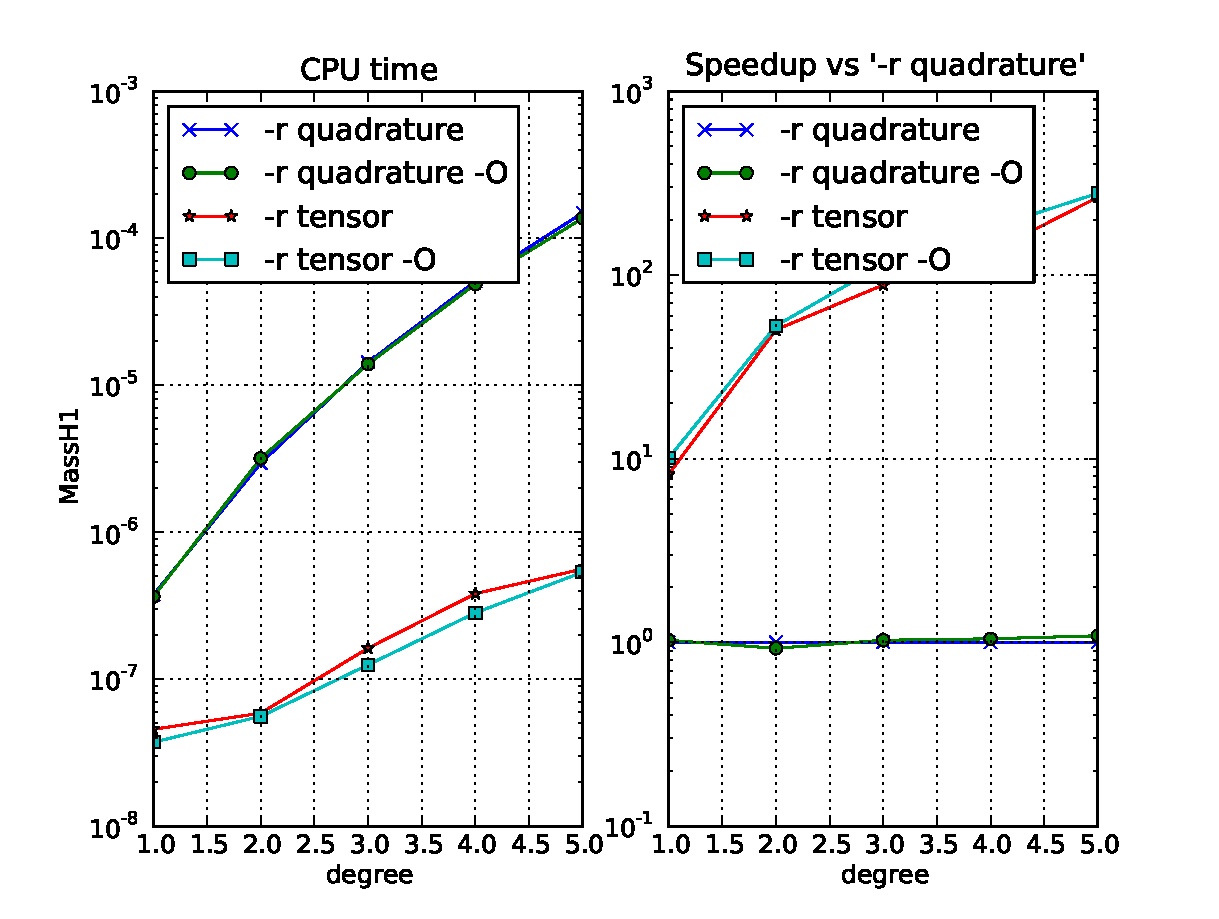
\includegraphics[width=\largefig]{chapters/kirby-3/pdf/MassH1.pdf}
  \caption{Speedup results for two-dimensional mass matrix using Lagrange polynomials.}
  \label{fig:MassH1}
\end{figure}

\subsection{Stiffness matrix for $H^1$}

Next, we consider the stiffness matrix on triangles defined by
\begin{equation}
  a(u, v) = \int_{\Omega} \nabla u \cdot \nabla v \dx,
\end{equation}
again using Lagrange elements of orders one through five. The speedup
results for this case are shown in Figure~\ref{fig:Poisson}.

\begin{figure}
  \centering
  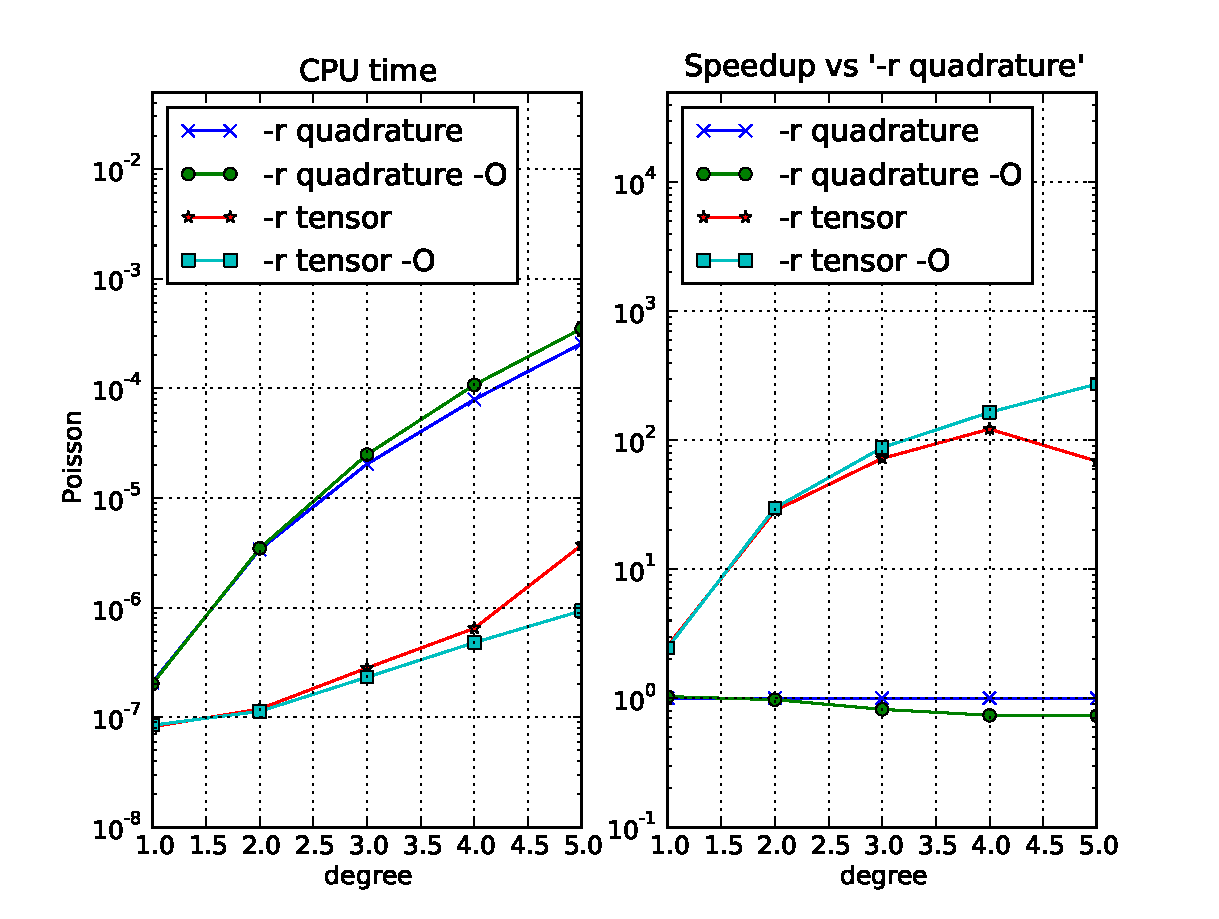
\includegraphics[width=\largefig]{chapters/kirby-3/pdf/Poisson.pdf}
  \caption{Speedup results for two-dimensional stiffness matrix using Lagrange polynomials.}
  \label{fig:Poisson}
\end{figure}

Again, we see that tensor contraction is preferred to quadrature for
this form. Unlike the mass matrix, we find that FErari optimizations
yield little result in the lowest order cases, but improve
significantly as the degree increases.

\subsection{Variable coefficient stiffness matrix}

We also consider the stiffness matrix with a variable coefficient,
\begin{equation}
  a(w; u, v) = \int_{\Omega} w \nabla u \cdot \nabla v \dx,
\end{equation}
where $ w $ lies in the same polynomial space as $ u $ and $ v$; that
is, Lagrange elements of orders one through five. The speedup results
are shown in Figure~\ref{fig:WeightedPoisson}.

\begin{figure}
  \centering
  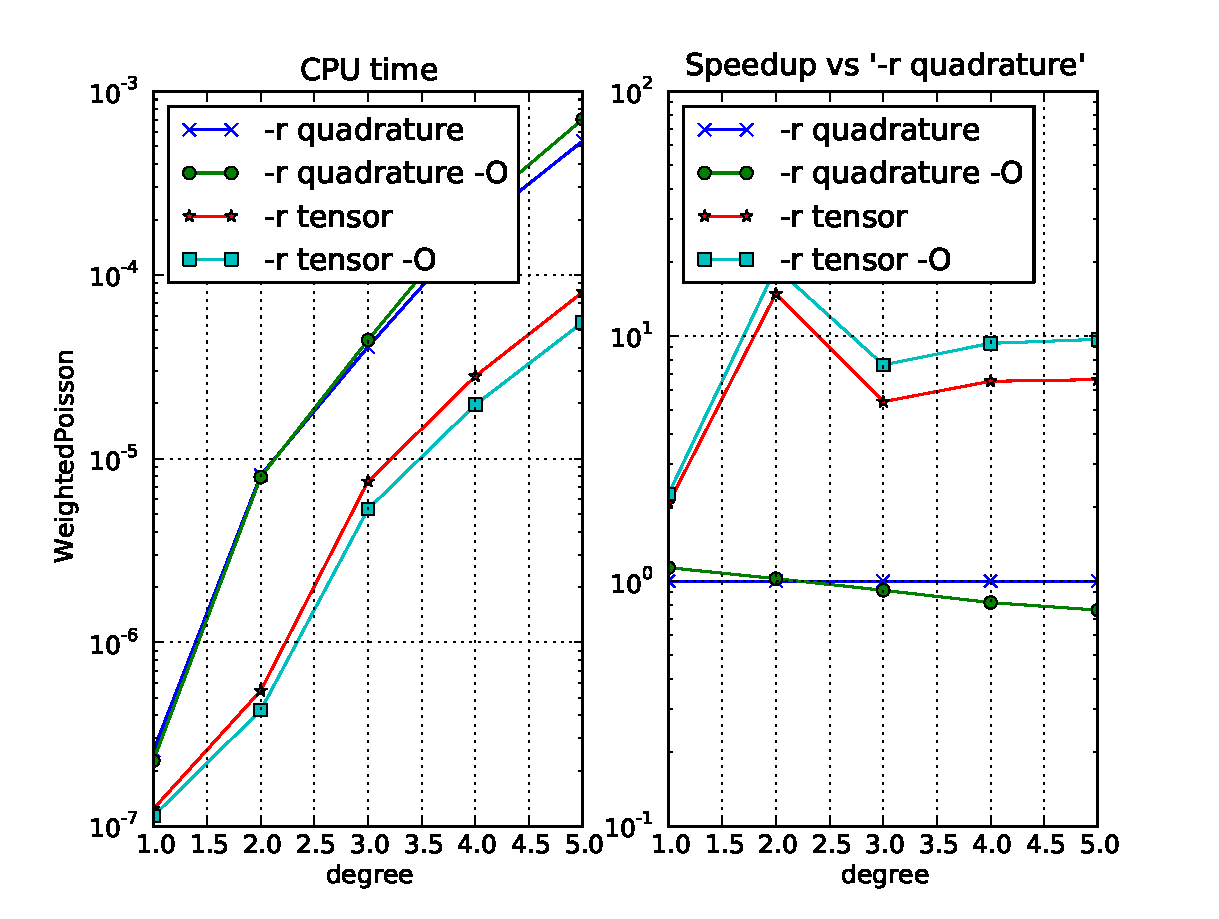
\includegraphics[width=\largefig]{chapters/kirby-3/pdf/WeightedPoisson.pdf}
  \caption{Speedup results for two-dimensional variable coefficient
    stiffness matrix using Lagrange polynomials.}
  \label{fig:WeightedPoisson}
\end{figure}
The difference between quadrature and tensor methods is smaller than
for the bilinear case with no coefficient, but tensor contraction is
still faster. FErari improves the tensor contraction by about 5-20\%
in each case.

\subsection{Navier--Stokes convective term}

Another problem where a variable coefficient taken from a finite
element space naturally arises is the Navier--Stokes equations. For
typical linearizations, one must evaluate the matrix associated with
the form
\begin{equation}
  a(w, \rho; u, v) = \int_T \rho \nabla u \, w \cdot v \dx,
\end{equation}
where $ w $ is taken from the same finite element space as $ u $ and $
v $, namely vector-valued polynomials. The function $ \rho $ is a
scalar-valued polynomial of the same degree as the other
functions. Such a function $ \rho $ will appear when one solves
problems with a spatially variable fluid density.

\begin{figure}
  \centering
  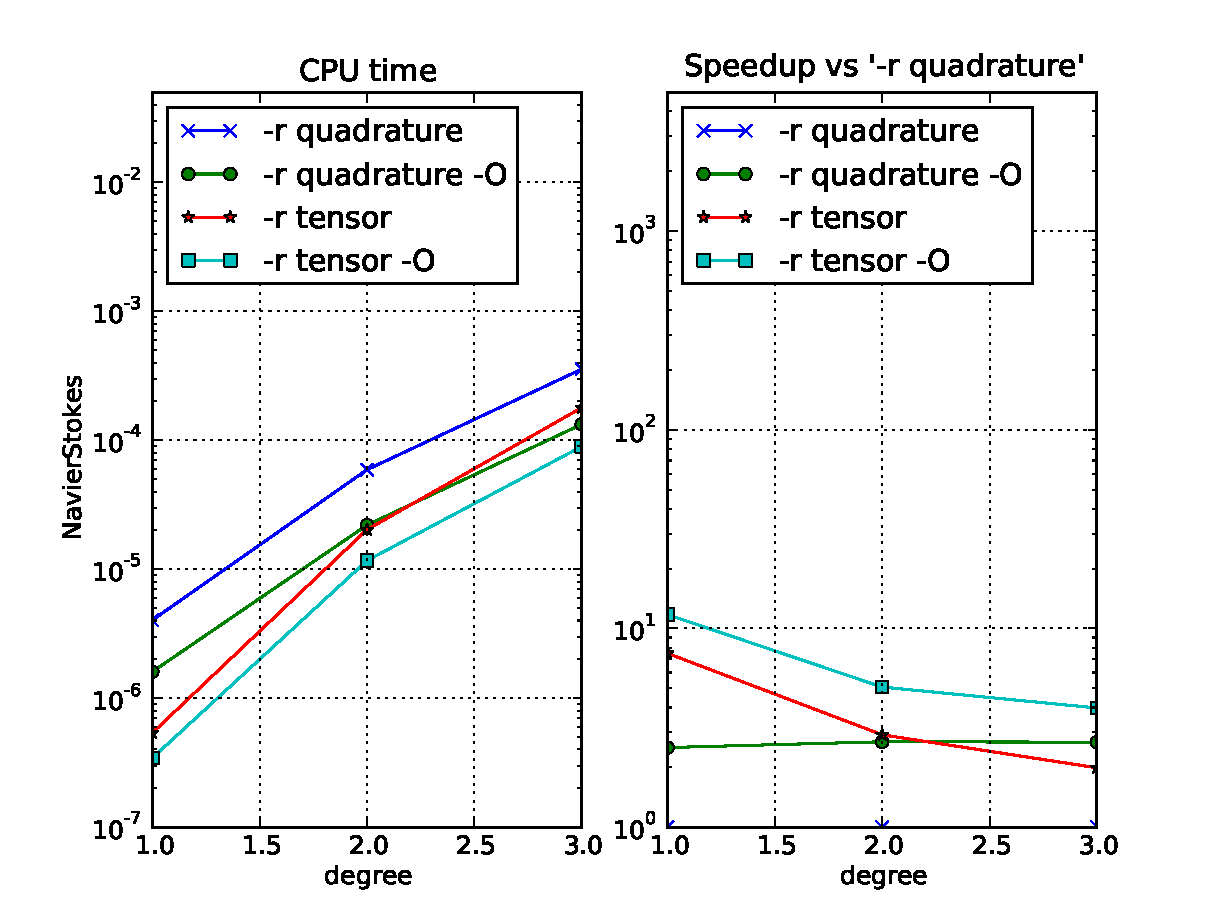
\includegraphics[width=\largefig]{chapters/kirby-3/pdf/NavierStokes.pdf}
  \caption{Speedup results for the two-dimensional convective term
    in Navier--Stokes using Lagrange polynomials.}
  \label{fig:NavierStokes}
\end{figure}

This problem is far more challenging than the previous ones and we
only consider up to cubic functions (not to exhaust system
resources). The two coefficient functions $ w $ and $ \rho $ tend to
make the quadrature-based methods more competitive with tensor
contraction.  Still, even for this more complicated form, FErari
delivered on the order of $ 10\% $ speedup over the tensor-based
method and outperforms quadrature.

\subsection{Mass matrices for $H(\mathrm{div})$ and $H(\mathrm{curl})$}

Next we consider again the mass matrix~\eqref{eq:MassH1}, but for $
H(\mathrm{div})$ and $H(\mathrm{curl})$ elements. For a discussion of
the treatment of the required Piola transforms,
see \citet{RognesKirbyLogg2009}. In these cases, the Piola transforms
make the computational pattern similar to the $ H^1 $ stiffness
matrix, but with different numerical values in the reference tensor
and hence potentially different speedup results for FErari. We
consider the Brezzi--Douglas--Marini elements of orders one through
five for $H(\mathrm{div})$ and the first kind \nedelec{} elements
for $H(\mathrm{curl}) $. The speedup plots are posted in
Figures~\ref{fig:MassHdiv} and~\ref{fig:MassHcurl}.

\begin{figure}
  \centering
  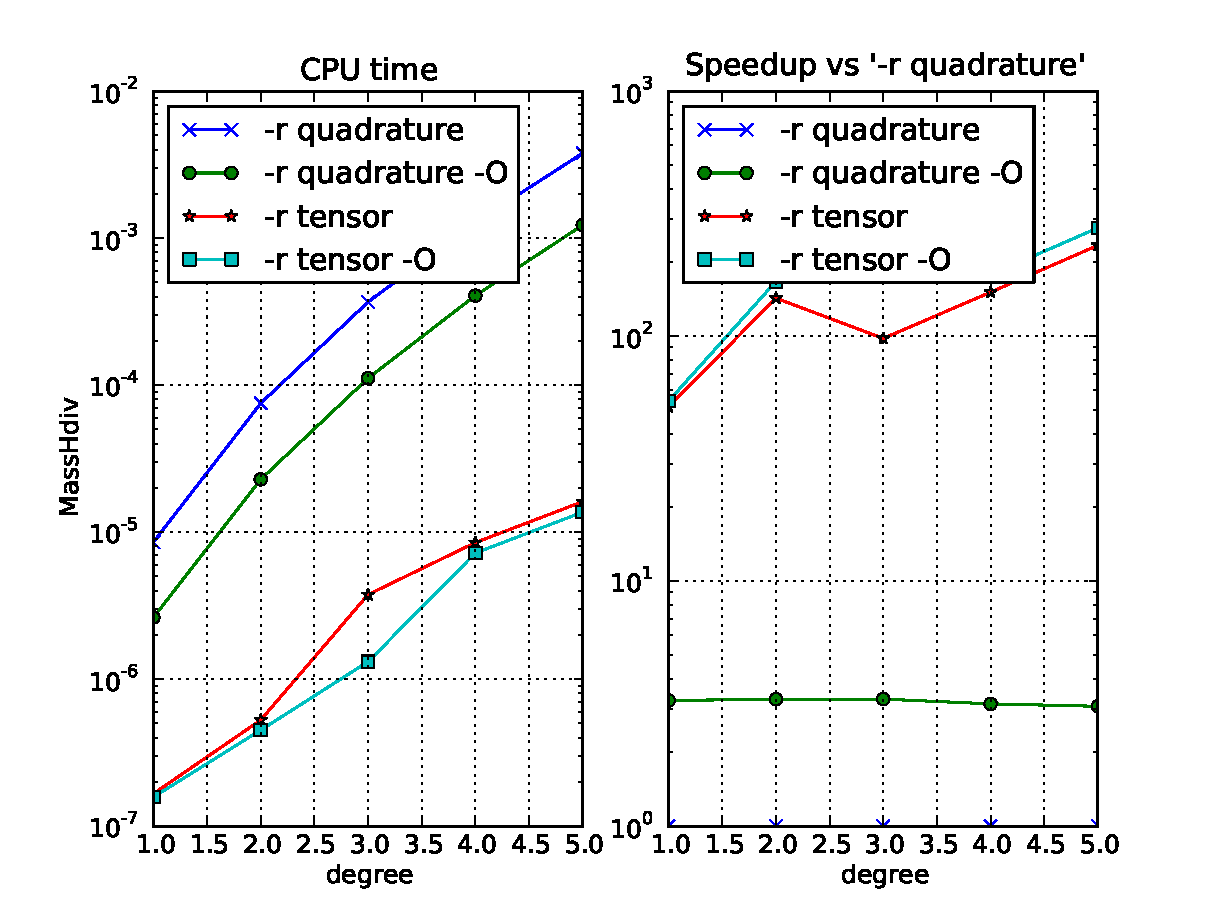
\includegraphics[width=\largefig]{chapters/kirby-3/pdf/MassHdiv.pdf}
  \caption{Speedup results for two-dimensional $H(\mathrm{div})$
    mass matrix  using BDM elements.}
  \label{fig:MassHdiv}
\end{figure}
\begin{figure}
  \centering
  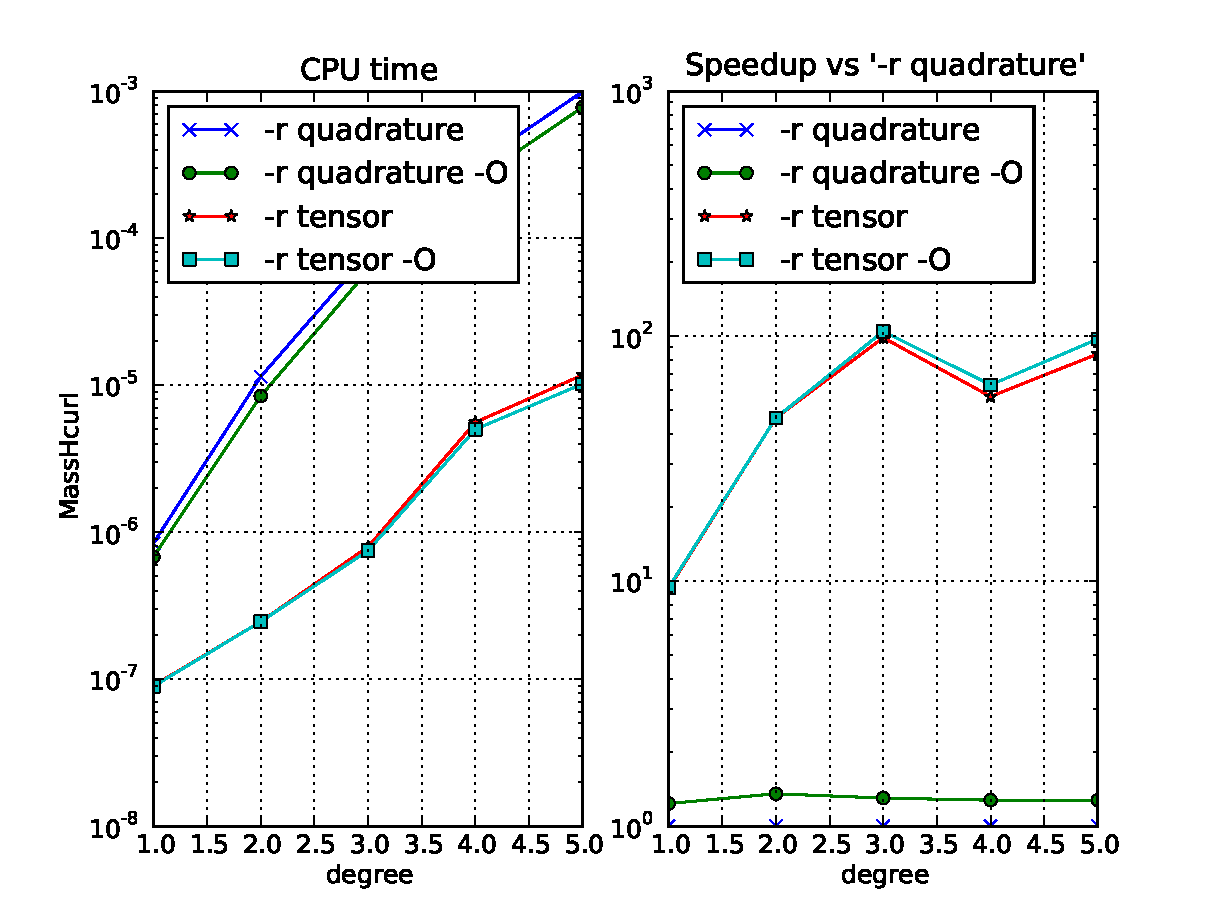
\includegraphics[width=\largefig]{chapters/kirby-3/pdf/MassHcurl.pdf}
  \caption{Speedup results for two-dimensional $ H(\mathrm{curl}) $
    mass matrix using \nedelec{} elements.}
  \label{fig:MassHcurl}
\end{figure}

Tensor contraction methods outperform quadrature methods for these
forms. For the $ H(\mathrm{div}) $ case, speedup of FErari over
standard tensor contraction ranges from a few percent to nearly a
factor of two. However, for $ H(\mathrm{curl}) $, FErari offers very
little speedup.

%------------------------------------------------------------------------------
\section{Conclusions}

We have studied a range of forms of various complexity. In most cases,
FErari-based optimizations provide modest to considerable speedup in
the run-time evaluation of variational forms. On the other hand, they
can greatly increase the time FFC requires to generate code and so are
less suitable for a development phase or a just-in-time compilation
strategy. As a general guideline, one may also state that quadrature
becomes more efficient relative to tensor contraction when the
complexity of a form increases as measured in the number of
coefficients and the number of differential operators, while the
tensor contraction approach is relatively more efficient for simple
forms and high order polynomials. Moreover, the construction of
cell tensors is only part of the overall consideration in making
finite element methods efficient.

%------------------------------------------------------------------------------
\section{Historical notes}

Support for FErari optimizations was introduced in FFC version 0.3.2
in 2006 but was lost in a later rewrite of FFC. Starting with
FErari~0.2.0 and FFC~0.9.1, which were released in 2010, FErari
optimizations are again supported in FFC.
